\chapter{Offline scheduling model}
\label{sec:offline_scheduling_model}

In this chapter, we will describe how the hierarchial topology representation can be used for solving offline scheduling problems. In offline scheduling, all information about jobs is known in advance, so the information about the exact weight, release and due times of all jobs is available to the scheduler.

\section{Motivational example for offline scheduling}
\label{sec:offline_scheduling_motivational_example}

We will start with a motivational example. Figure \ref{fig:offline_scheduling_topology} shows the topology for this example, and figure \ref{fig:offline_scheduling_jobs} shows the jobs paths DAGs for three jobs which need to be processed in the system. In this figure, every paths DAG node is assigned a number, which we will call \textit{step identificator}. The motivation behind introducing the \textit{step identificator} is that the information \textit{(job identificator, machine identificator)} can be ambiguous, because jobs can be processed on the same machines multiple times. Instead, a concept of a processing step is introduced, which corresponds to a single instance of processing a job on a machine, and each node in the job's paths DAG is equivalent to one step.

\begin{figure}[!htbp]
	\centering
	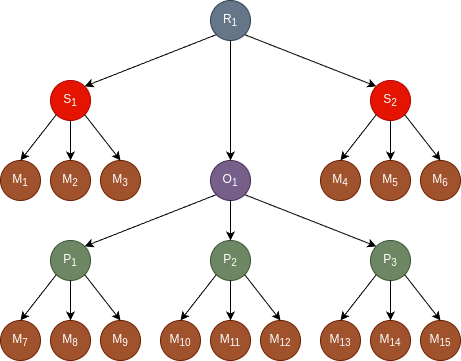
\includegraphics[scale=0.6]{../images/offline_scheduling_topology.png}
	\caption{Offline scheduling motivational example - topology}
    \label{fig:offline_scheduling_topology}
\end{figure}

\begin{figure}[!htbp]
	\centering
	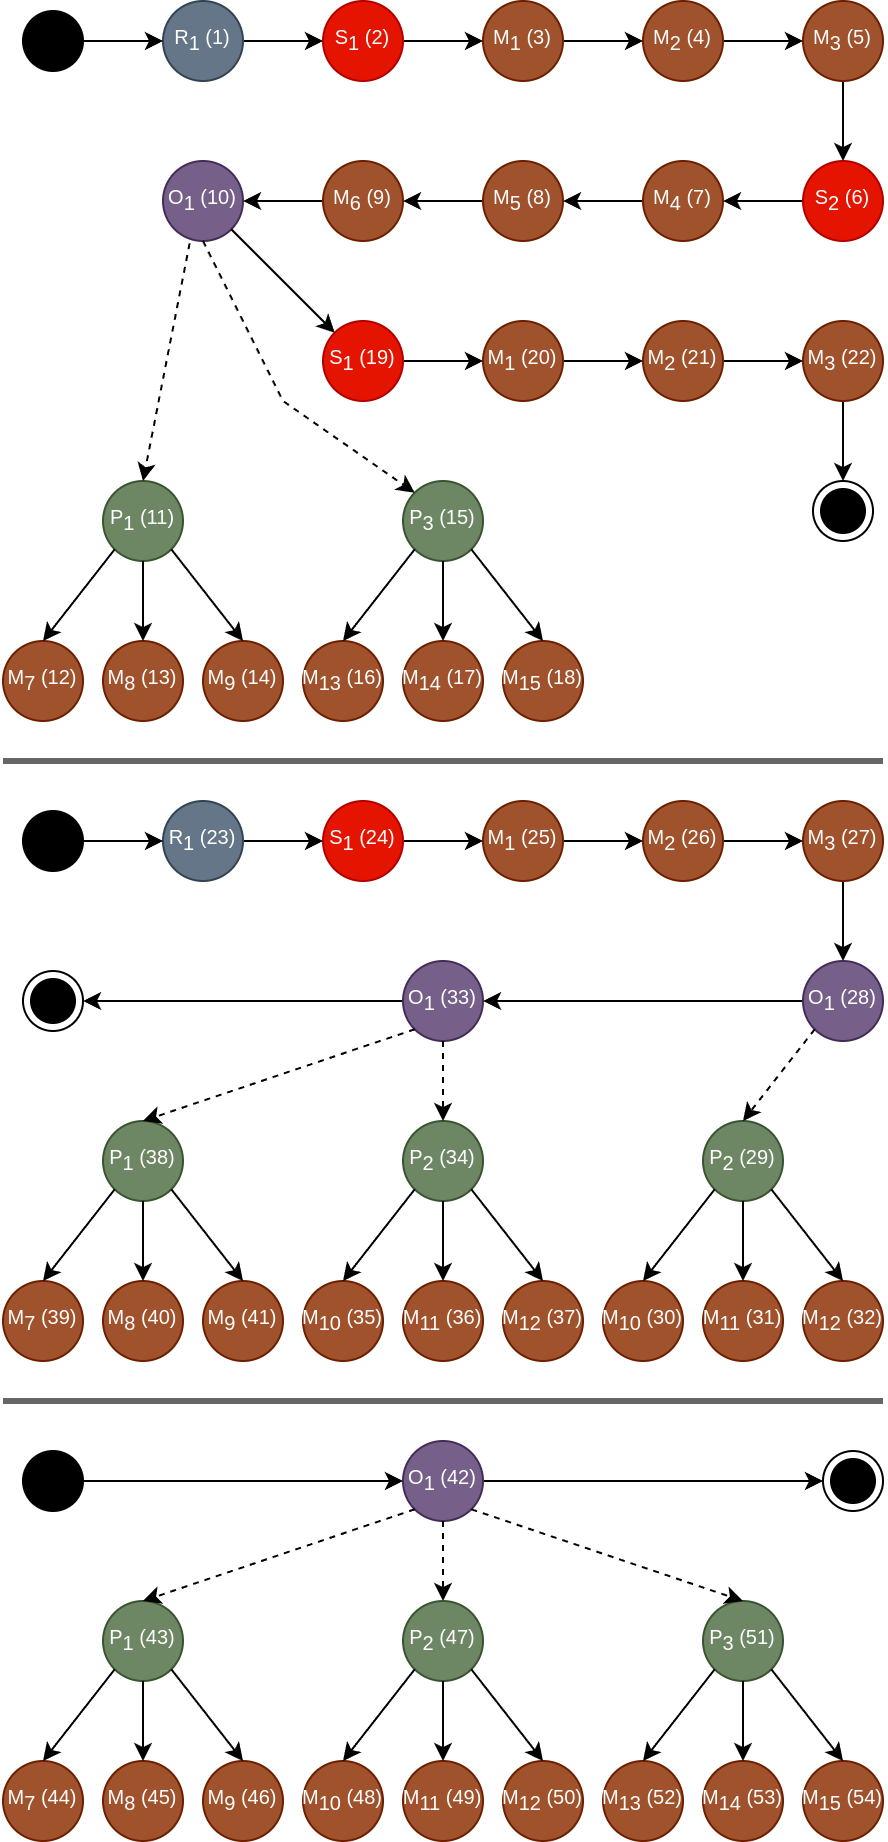
\includegraphics[scale=0.6]{../images/offline_scheduling_jobs.png}
	\caption{Offline scheduling motivational example - jobs paths DAGs}
    \label{fig:offline_scheduling_jobs}
\end{figure}

\section{Offline scheduling genotype components}
\label{sec:offline_scheduling_genotype_components}

Next, we will consider what it means to do scheduling in an environment where all information about jobs is available to the scheduler. Looking at our motivational example, we can extract some key points.

Firstly, we know the basic information about jobs - release time, due time, weight. This means that for each job, we know how important it is, when it will become available for processing, and by what time we should finish its processing.

Secondly, we know all the possible paths that each job can take through the system. We can gather this information from the job's paths DAG. In practice, this DAG would be constructed from the job's processing requirements and restrictions.

In a hierarchial topology, scheduling happens on two levels. The first one is determining a job's processing route, and the second one is determining the order in which the jobs are processed on machines.

\subsection{Offline scheduling genotype - processing routes}

First, we will focus on the processing routes. This happens in the inner nodes of the topology tree. For the serial group, no scheduling is done, as the group rules dictate that every job will be processed on the group's first component, then second, all the way to the final one. The same is true for the route group, where for each job, it is predetermined which route it will take through its components.

For the parallel group, which has of several components, and each job has to go through exactly on of them, it is the scheduler's job do decide which one the job will go through. This is the first component of an offline schedule genotype. For each job, for each path node which corresponds to a parallel group in the topology, all of its successor nodes are placed in a list, and among them one is chosen as the node the job will go through. This part of the genotype is shown in figure \ref{fig:offline_scheduling_genotype_parallel}. For three jobs, there are eight parallel group nodes, and for each them, the successor is shown in a darker color, with the remaining nodes being colored lightly.

\begin{figure}[!htbp]
	\centering
	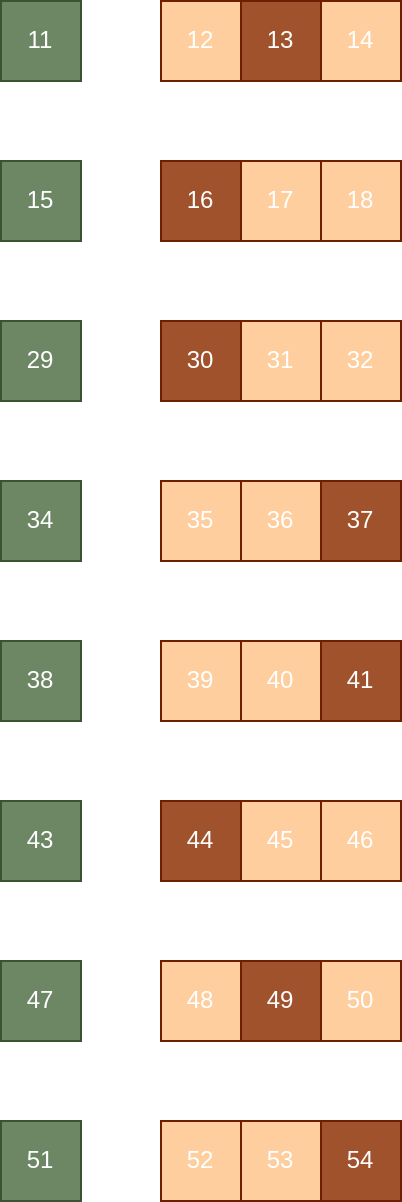
\includegraphics[scale=0.6]{../images/offline_scheduling_genotype_parallel.png}
	\caption{Offline scheduling example - genotype for parallel groups}
    \label{fig:offline_scheduling_genotype_parallel}
\end{figure}

For the open group, which also has of several components, and each job has some components it has to go through, but no restriction is imposed on the order that the job will go through them, it is the scheduler's job to determine this order. This is the second component of an offline schedule genotype. For each job, for each path node which corresponds to an open group in the topology, all of its successors are placed in a list, and the order of the components in this list dictates the order in which the job will go through the path nodes. This part of the genotype is shown in figure \ref{fig:offline_scheduling_genotype_open}. For three jobs, there are four open group nodes, and for each them, the traversal order of their successors is shown.

\begin{figure}[!htbp]
	\centering
	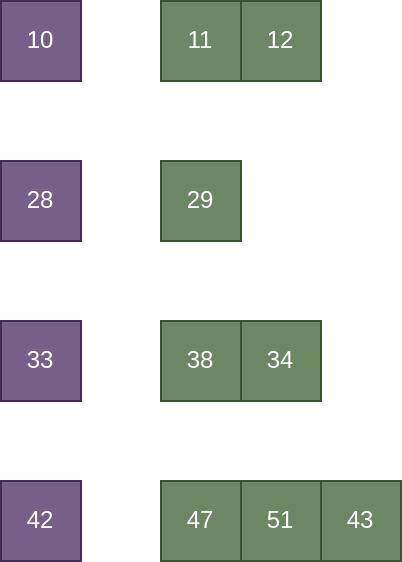
\includegraphics[scale=0.6]{../images/offline_scheduling_genotype_open.png}
	\caption{Offline scheduling example - genotype for open groups}
    \label{fig:offline_scheduling_genotype_open}
\end{figure}

\subsection{Offline scheduling genotype - processing orders}

Next, we will focus on the second level of scheduling, which is determining the order in which the jobs are processed on machines. This is the third and final component of an offline schedule genotype. For each machine, it is precalculated which processing steps can happen on it. These steps are placed in a list, and the order of this list determines the order of processing on the machine. How this works in practice is that, in the machine's buffer, jobs are ordered using the order in the genotype, and every time the machine can start processing a job, it takes the first step from the buffer and starts its processing. This part of the genotype is shown in figure \ref{fig:offline_scheduling_genotype_machine}.

\begin{figure}[!htbp]
	\centering
	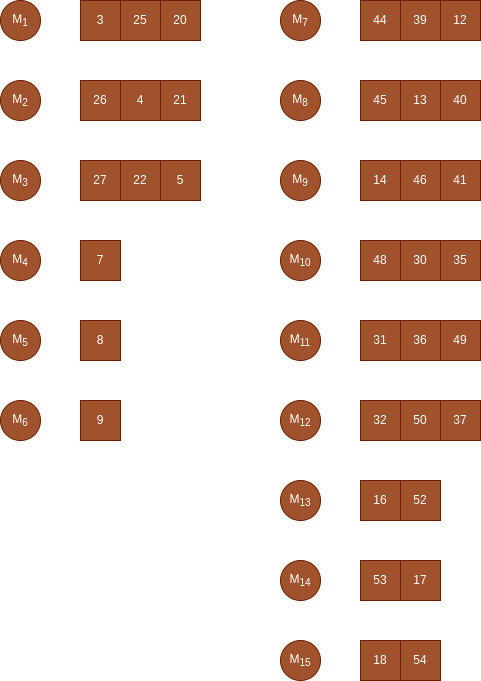
\includegraphics[scale=0.6]{../images/offline_scheduling_genotype_machine.png}
	\caption{Offline scheduling example - genotype for machines}
    \label{fig:offline_scheduling_genotype_machine}
\end{figure}

\subsection{Offline scheduling genotype - passive components}

These three components build an offline schedule genotype. An important note to make is that the genotype can contain passive components, by which we mean that they do not impact the scheduler and its decisions. 

One way that this can happen is if the topology contains parallel groups. All branches of these groups are covered by the genotype, but only one will be relevant for each job that goes through the parallel group. If a passive branch of a parallel group node contains an open group, then the order of its component nodes in the genotype will be irrelevant, until the branch becomes active by changing the parallel group node in the genotype. 

Another way in which a component of a genotype can be passive is for machines, where the genotype for each machine will be fully utilized only if all its processing steps are waiting in its buffer at the same time. Otherwise, changing the order of steps for a machine can have no impact on the order in which the steps are processed.

\section{Offline scheduling genotype operators}
\label{sec:offline_scheduling_genotype_operators}

In chapter \ref{sec:offline_scheduling_genotype_components}, we have presented the genotype for offline scheduling. In this chapter, we will present all of its operators, and this will make the offline scheduling genotype compatible and optimizable with the framework presented in chapter \ref{sec:optimization_model}.

\subsection{Offline scheduling genotype - evaluation function}
\label{sec:offline_scheduling_genotype_evaluation_function}
The evaluation model for the hierarchial topology representation was explained in chapter \ref{sec:evaluation_model}. To reiterate, the processing of a job sequence is simulated, and the simulation yields some data about each job. Then, an objective function is calculated using the job data, and the result represents the schedule score. This exactly is the evaluation function for the offline scheduling genotype - run a simulation, collect results, pass them to an objective function and calculate the schedule score. The two parameters of an evaluation function are the job sequence and the objective function, and changing them produces different evaluation functions.

\subsection{Offline scheduling genotype - creation operator}
The genotype for offline scheduling consists of three components, as described in chapter \ref{sec:offline_scheduling_genotype_components}. All genotype operators manipulate all of these components. Before the optimization, paths DAGs of all jobs are analyzed, to collect information about all possible scheduling decisions that could be made. For each machine, a list of all processing steps which could be executed on it is compiled. For parallel and open groups, all path nodes are compiled.

For machines, a creation operator constructs a random permutation of all steps which are to be executed on the machine. For parallel group nodes, a creation operator randomly chooses one of its components. For open group nodes, a creation operator constructs a random permutation of all components the job has to go through.

\subsection{Offline scheduling genotype - combination operator}
For parallel group nodes, a combination operator takes the genetic material from one of the parents. For open group nodes and machines, any combination operator for a permutation representation can be used, and several are described in \citep{cicirello2023ecta} as \textit{crossover operators}.

\subsection{Offline scheduling genotype - perturbation operator}
For parallel group nodes, a perturbation operator works in the same way as a creation operator - it randomly chooses on of the group's components. For open group nodes and machines, any perturbation operator for a permutation representation can be used, and several are described in \citep{cicirello2023ecta} as \textit{mutation operators}.

\subsection{Offline scheduling genotype - neighborhood operator}
For simple representations, a complete and exhaustive neighborhood operator can be constructed. One such representation is a binary vector representation, which consists of $n$ numbers, each one being $0$ or $1$. A neighborhood operator could flip the value at each position, and thus produce $n$ neighbors.

For more complex representations, exhaustively listing all neighbors becomes intractable. For such representations, a neighborhood operator can be simulated by using the perturbation operator $n$ times and returning all perturbations as the list of neighbors. This is the approach that we will use for the offline scheduling genotype, and all the remaining genotypes that will be explained throughout this thesis. Where a neighborhood operator is not explicitly defined, it is assumed that a perturbation operator is used as its surrogate.

\section{Topology partitioning}
\label{sec:topology_partitioning}

We have seen that an offline scheduling genotype consists of $a$ machine step permutations, $b$ parallel group node selections and $c$ open group node permutations. We have also decribed how genotype operators transform each of these genotype components. The question that is left to answer is which of these components are being transformed at any moment when an operator is being applied.

For this purpose, we will introduce the concept of topology partitioners. At certain moments during optimization, a topology partitioner will be invoked to generate a new subset of components, and only components in this subset can be altered until the next invocation of the partitioner, while the remaining components stay fixed. Next, we will describe several partitioners which we will use later.

A \textit{basic partitioner} always returns all components.

A \textit{start to end partitioner} organizes all components in a list, where the components are ordered by the topological order of their respective topology components. Each time that this partitioner is invoked, it returns $k$ components, where $k$ is a parameter which defines how many components can be changed at once. The partitioner iterates through all components from start to end with a step $k$, and when it reaches the end, it circles back to the beginning of the components list.

An \textit{end to start partitioner} works similarly to the \textit{start to end partitioner}, but it iterates through the components list from the end to the beginning. Everything else works in the same way for both partitioners.

A \textit{fair random partitioner} creates a random permutation of all components, and iterates through it from start to end with a step $k$, similarly to the \textit{start to end partitioner}. When it reaches the end of the permutation, it creates a new one. It is random because the order in which the components are changed is random, and it is fair because all components are changed roughly the same number of times.

A \textit{true random partitioner} returns $k$ random components any time it is invoked. Unlike the \textit{fair random partitioner}, there is no guarantee that components will be changed in a fair way, because they are chosen completely randomly every time that a new partition is created.

Finally, a \textit{random path partitioner} creates a random path through the topology, and returns all components on the path. When it reaches a route or open group element, it includes each of its components with a chance $p$, which is its parameter.

Next, we will discuss how the introduction of topology partitioners affects the genotype operators. The only operators which are affected are the perturbation and combination operators.

For perturbation operators, the components which are open for change are perturbated, while the remaining ones are fixed. 

For combination operators, the components which are open to change are constructed using the combination operators for the component. Since a combination operator creates a new genotype from two parent genotypes, this creates a problem in constructing new genotypes, as it is not clear how to create components which are fixed and can not be changed at the time. For this purpose, we will introduce combination operators with coarse and fine granularity. The coarse granularity operator randomly chooses a parent, and copies all fixed components from that parent. The fine granularity operator chooses a random parent for each fixed component, and copies the component from it.

\section{Scheduling meta-algorithm}
\label{sec:scheduling_meta_algorithm}

We can now describe the algorithm which we will use to do optimization for both offline and online scheduling. The algorithm is called \textit{scheduling meta-algorithm}, and its pseudocode can be found in algorithm \ref{alg:sma}.

The algorithm has two evaluation functions. The first function contains the sequence of jobs used for training, and the second function contains the sequence used for testing. This is analogous to the concepts of \textit{train sets} and \textit{test sets} in machine learning.

In the inner loop of the algorithm, an optimization algorithm searches the solution space for a good solution, evaluating the solutions on the train set. Any algorithm described in chapter \ref{sec:optimization_algorithms} can be used as the inner optimization algorithm.

In the outer loop of the algorithm, a topology partitioner is used to create a new partition of components that will be changed in the inner loop of the algorithm, the inner algorithm is called, and its result is evaluated using the test set. 

It is important to note that the population of solutions is transferred from one call of the inner algorithm to the next one. In each iteration, the topology partitioner determines which components of the genotype will be changed, while the others remain constant. This property allows the algorithm  to change only some parts of the solutions and keep the remaining ones frozen, thus exploring the solution space in a controlled way.

\begin{algorithm}[!htbp]
    \caption{Scheduling meta-algorithm}
    \label{alg:sma}
    \KwIn{$evaluation\_function\_train$, $evaluation\_function\_test$, $creation\_operator$, $combination\_operator$, $perturbation\_operator$, $topology\_partitioner$, $inner\_algorithm$, $number\_of\_iterations$}
    \KwOut{$(best\_solution, best\_score)$}

    $x \gets creation\_operator.create()$\;
    $s \gets evaluation\_function\_test.evaluate(x)$\;
    $population \gets creation\_operation.createPopulation()$\;

    \For{$iter \gets 1$ \KwTo $number\_of\_iterations$} {

        $machines\_partition = topology\_partitioner.getPartition()$\;
        $(x', \_)$ $\gets$ $inner\_algorithm.optimize($$evaluation\_function\_train,$ \newline \hspace*{1em} $creation\_operator$, $combination\_operator$,  $perturbation\_operator,$\newline \hspace*{1em}$ machines\_partition, population)$\;
        $s' \gets evaluation\_function\_test.evaluate(x')$\;
        \If{$s' < s$}{
            $(x, s) \gets (x', s')$\;
        }
    }

    \Return $(x, s)$\;
    \end{algorithm}

\section{Case study: scheduling university laboratory exercises}
\label{sec:case_study_lab}

In this chapter, we will describe how to use the offline scheduling representation to solve to problem of scheduling university laboratory exercises. The premise of the problem is that a total of $x$ students are enrolled in an university course, and they all need to pass a laboratory exercise, which is being held in $y$ different slots. The goal is to assign each student to a slot, while satisfying some constraints - each slot has a capacity of students that cannot be exceeded, and student cannot have conflicts in their university timetables.

This is an interesting problem, because it is not immediately evident how to solve this problem using the concepts explained in this chapter. But it is important to remember that scheduling is the process of allocating resources to tasks. In the model of machines and jobs, machines are resources, and jobs are tasks. In the problem of scheduling university laboratory exercises, slots are resources, and enrolled students are tasks.

Let's imagine that the exercises are organized in five different slots, three being on one day, and two being on another. On the first day, three teaching assistants are available for exercises, while on the second day, only two of them are available. Each assistant can process a maximum of ten students per slot. This means that the first three slots can have a maximum of $30$ students, while the last two can have a maximum of $20$ students. Let's also imagine that a total of 124 students are enrolled in the course.

We will also assume that the slots for exercises are defined in advance. If the slots should also be scheduled, then the problem would require scheduling on two levels - scheduling timeslots, and scheduling students to fixed timeslots. For simplicity, we will cover only the second subproblem and assume that the slots are determined by a human, which is a reasonable assumption.

For each student, we need to choose one of five available slots. This can be represented using a parallel group component. The proposed topology and paths DAG are shown in figure \ref{fig:case_study_lab}. We can assume that the machines $M_1$, $M_2$ and $M_3$ can process $30$ students in batch, while the machines $M_4$ and $M_5$ can process $20$ students.

\begin{figure}[!htbp]
	\centering
	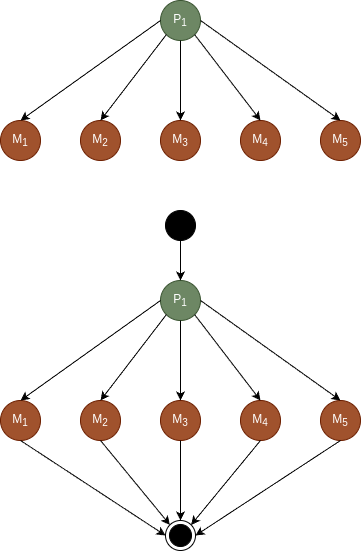
\includegraphics[scale=0.6]{../images/case_study_lab.png}
	\caption{Scheduling university laboratory exercises - topology and paths}
    \label{fig:case_study_lab}
\end{figure}

A hard constraint of the problem is that the student has no collisions in their timetable. A number of soft constraints for the problem could be defined, for example, a student does not have gaps larger than two hours in their timetable, or the student does not have to spend more than eight hours per day at university. If a solution does not satisfy a hard constraint, it is invalid. Solutions which satisfy all hard constraints can be compared in a way that those which satisfy more soft constraints are better. The goal is to ensure that no students have collisions in their timetables, and that as few students as possible have large gaps in their timetables or long days at the university.

The evaluation function would analyze the timetable of each student, and the score for a student is calculated based on whether the hard constraint is satisfied, and how many soft constraints are satisfied. Scores for all students are summed, and that is the score for the schedule.

The creation operator would randomly assign students to slots, respecting the constraints that first three slots can have no more than $30$ students, and the remaining two slots can have no more than $20$ students.

The combination operator would, for each student, randomly choose the assigned slot from one of the parents. The problem that arises is that applying this operator could break the hard constraint of the maximum number of students per slot. This can be solved by applying a greedy randomized heuristic that fixes the solution obtained from the combination operator. It would move students from the overfilled slots to the underfilled ones, using some randomized heuristic criteria.

The perturbation operator would swap the assigned slots for a randomly chosen pair of students $k$ times.

Finally, the optimization algorithm could be the \textit{scheduling meta-algorithm} if we want to utilize \textit{topology partitioners}, or any algorithm from the chapter \ref{sec:optimization_algorithms} if we want to change all slots in each iteration of the algorithm. 

In this case study, we have described, on a high level, how to use the offline scheduling representation to solve a problem of scheduling university laboratory exercises. This was an exercise of analyzing the limited resources and tasks in the problem, and applying the concepts of machines and jobs to this view of the problem. These concepts can be applied to a variety of problems, and thus, the offline scheduling representation could be used to solve such problems.

\chapter{Online scheduling model}
\label{sec:online_scheduling_model}

\section{Comparison with offline scheduling}

In this chapter, we will describe how the hierarchial topology representation can be used for solving online scheduling problems. In online scheduling, the information about jobs, such as their count and properties, is not known in advance. Instead, as the jobs enter the system, the scheduler dynamically moves them across the system.

\section{Online scheduling genotype components}
\label{sec:online_scheduling_genotype_components}

In chapter \ref{sec:offline_scheduling_model}, we have described the model for offline scheduling. The majority of the concepts presented for offline scheduling apply for online scheduling as well, including the topology partitioners and scheduling meta-algorithm. The only difference lies in how the scheduler makes decisions.

In offline scheduling, all scheduling decisions were made in advance. For each job, its path through the system was defined. For each machine, the preferred processing order of jobs was defined. In online scheduling, these decisions will be made dynamically.

\subsection{Online scheduling genotype - processing routes}

When a job is processed on a parallel machine, the scheduler needs to determine which machine the job will be processed on next. In offline scheduling, this decision is made by reading the genotype. In online scheduling, this decision is made by manipulating some features to determine the best branch of the parallel machine to enter. This problem can be framed as a classification problem. In that case, each parallel machine would have a classifier which would determine the most suitable branch.

Things get a bit more complicated when we consider online scheduling for open groups. Defining this problem as a classification problem does not make sense, because for each job, the branches of the group to select from could be different. Let's imagine that a job has $m$ components of the open group to go through. When it first arrives at the group, it is the scheduler's decision to choose which of these $m$ components the job will go through first. When the job finished with the first component, the scheduler needs to decide which of the remaining $m-1$ components the job will go through next. After that, the scheduler needs to choose one of the $m-2$ components, and this goes all the way until the job goes through all the components. So, the order of components for a job is not determined at one moment, and instead, it is constructed part by part, at different moments of the simulation.

Since framing the problem as a classification problem does not make sense for open groups, for the sake of uniformity, we will frame the problem for both parallel and open groups as a regression problem. In parallel groups, using some features, the scheduler will assign a score to each branch. The branch with the highest score is the one that the job will go through. The same applies for open groups - any time that a scheduler needs to choose which of the $k$ components a job will go through next, it will calculate a score for each of them, and the job will go through the one with the highest score. The goal of the regression algorithm is to determine how good a component of a group is, and in both the cases of parallel and open groups, the best component is chosen.

\subsection{Online scheduling genotype - processing order}

When a scheduler needs to decide which of the jobs in the machine's buffer it will process next, it will calculate the score for all of the jobs, and the job with the highest score is the one which will be processed next. The problem to solve here is a regression problem, where the goal is to determine how important a job is in the context of a machine, and the most important job gets processed first.

\section{Online scheduling features}
\label{sec:online_scheduling_features}

In chapter \ref{sec:online_scheduling_genotype_components}, we presented components of an online scheduling genotype. In offline scheduling, the genotype consists of three different categories - parallel groups, open groups and machines. In online scheduling, the genotype is more elegant. Every element of the topology which requires some form of scheduling has a regression algorithm, and the outputs of this algorithm are interpreted according to the element rules. In this chapter, we will define the features that the regression algorithms will have at their disposal to calculate the score of a job or a branch.

\subsection{Processing routes features}

For paralell and open groups, where the regression algorithm needs to evaluate how good a component of the group is for the job, the features that the algorithm can use are the following:
\begin{itemize}
    \item time (timestamp at which the job is processed on the group)
    \item job's release time
    \item job's due time
    \item job's weight
    \item job's remaining processing time in the branch
    \item the number of jobs which have entered the component
    \item the number of jobs which are currently in the component and all its descendants
    \item whether the component has free space in its buffer
    \item whether all the prerequisites for the job's processing on that component are satisfied
  \end{itemize}

\subsection{Processing order features}

For machines, where the regression algorithm needs to evaluate how important a job is relative to the machine, the features that the algorithm can use are the following:
\begin{itemize}
	\item time
	\item job's release time
	\item job's due time
	\item job's weight
	\item combined weights of all the jobs that the job is batch compatible with (can be processed in batch with)
	\item number of batch compatible jobs for the job
	\item batch processing limit (maximum number of jobs per batch) for the machine type and job type pairing
	\item setup length of the job for the machine, relative to the job which was previously processed on the machine
	\item time until the machine's next breakdown
	\item whether preemptions are allowed for the machine type and job type pairing
\end{itemize}

\section{Online scheduling limitations}
\label{sec:online_scheduling_limitations}

In this chapter, we will go over some limitations of the online scheduling model presented in this chapter.

For open groups, each time that the scheduler needs to choose the next group's component for the job, the regression algorithm for the group is executed once for each remaining component. This means that, if a job has to go through $m$ components on the open group, a total of $m + (m - 1) + (m - 2) + ... + 3 + 2$ calculations are required, which has the complexity of $O(m^2)$. This is poorly scalable, and becomes a problem if the job has a significant number of components per an open group to go through.

Similarly, for machines, each time that the scheduler needs to choose the next job to be processed on the machine, the regression algorithm for the machine is executed once for each job in the machine's buffer. If the machine's buffer can have at most $n$ jobs at any moment, and a total of $m$ jobs have to be processed on the machine, the complexity for these calculations is $O(mn)$, which is also poorly scalable.

A potential solution for this problem is to execute the regression algorithm once per component for open groups, and once per job for machines. A tradeoff is made here - processing complexity is reduced from $O(m^2)$ to $O(m)$, but the scheduler now works with outdated information. 

To remedy the problem of outdated information, an adjustment coefficient could be introduced. This would be a function of all the parameters of a regression problem. The score of a job for machines and components for open groups would become the product of the output of their respective regression algorithm and the adjustment coefficient, which could be trained in a similar way as regression algorithms. For example, for jobs in a machine's buffer, the adjustment coefficient could assign higher values to jobs which arrive earlier at the machine, thus prioritizing jobs which have waited more in the buffer.

However, in this thesis, we will not explore these concepts further, and will instead stick to the calculation models presented in the chapter \ref{sec:online_scheduling_features}. These ideas could be explored in future work.

\section{Online scheduling algorithm cluster}
\label{sec:online_scheduling_algorithm_cluster}

As we discussed earlier in this chapter, each element of the topology which requires some scheduling decisions will have a regression algorithm assigned to it. We will refer to the collection of these algorithms as the \textit{online scheduling algorithm cluster}, and a single regression algorithm will be referred to as \textit{online scheduling algorithm}.

The online scheduling algorithm cluster is the genotype for an online scheduling problem. In this chapter, we will go over its operators.

\subsection{Online scheduling algorithm cluster - evaluation function}
The evaluation function for an online scheduling algorithm cluster is the same as the evaluation function for the offline scheduling genotype, described in the chapter \ref{sec:offline_scheduling_genotype_evaluation_function}. The steps are - simulate the processing of a job sequence in the system, produce some data about each job, and aggregate this data to a single value using an objective function.

\subsection{Online scheduling algorithm cluster - creation operator}
The creation operator for an online scheduling algorithm cluster involves creating an online scheduling algorithm for each topology element that requires scheduling. This involves calling the creation operator for the online scheduling algorithm once per select topology elements.

\subsection{Online scheduling algorithm cluster - combination operator}
The combination operator for an online scheduling algorithm cluster involves calling the combination operator of the online scheduling algorithm once per topology elements unlocked by the topology partitioner, and for the topology elements which are locked by the topology partitioner, the approach which was described in chapter \ref{sec:topology_partitioning} is used, with the distinction of coarse and fine granularity combination operators.

\subsection{Online scheduling algorithm cluster - perturbation operator}
The perturbation perturbation operator for an online scheduling algorithm cluster involves calling the perturbation operator of the online scheduling algorithm once per topology elements unlocked by the topology partitioners, while the remaining elements are left intact.

\section{Online scheduling algorithms}
\label{sec:online_scheduling_algorithms}

In this chapter, we will describe the online scheduling algorithms which can make up an online scheduling algorithm cluster. An online scheduling algorithm is a genotype for solving a regression problem. In chapter \ref{sec:online_scheduling_algorithm_cluster}, we described the operators for an online scheduling algorithm cluster. The majority of these operators assume that the online scheduling algorithms have the operators of the same type defined. Based on this information, we can conclude that each online scheduling algorithm needs to have creation, combination and perturbation operators defined. Furthermore, each online scheduling algorithm needs to be able to map a set of numeric features to a number, and in this way solve a regression problem.

\subsection{Random programming}

Random programming (RP) is a simple algorithm which maps a set of features to a random number. This means that a choice of a component in a parallel group is random, the processing order of components in an open group is random, and the processing order of jobs on machines is random. It does not have any associated data structures, so all its operators are trivial. The motivation behind naming is that the majority of online scheduling algorithms which we will use will be genetic programming algorithms.

\subsection{Neural network}

Neural network (NN) \citep{nn} is an universal approximator, and in this thesis, we will limit ourselves only to feedforward networks. An illustration of a neural network is shown in figure \ref{fig:nn}. In this figure, a bias vector and a linear transformation are combined in a single affine transformation. White square elements have value $0$, gray square elements have value $1$, blue square elements correspond to a linear transformation, green square elements correspond to a bias vector, and red square element correspond to result vectors after each transformation.

The creation operator for NN creates random affine transformation matrices, and the values are generated from a normal distribution. The combination operator for NN is the arithmetic mean across all affine transformations. The perturbation operator for NN adds random Gaussian noise to all affine transformations. The regression algorithm for NN is the forward pass.

Hyperparameters for NN are the standard deviations for Gaussian distributions used in the creation and perturbation operators (mean is $0$), nonlinear activation function and the architecture of hidden layers.

\begin{figure}[!htbp]
	\centering
	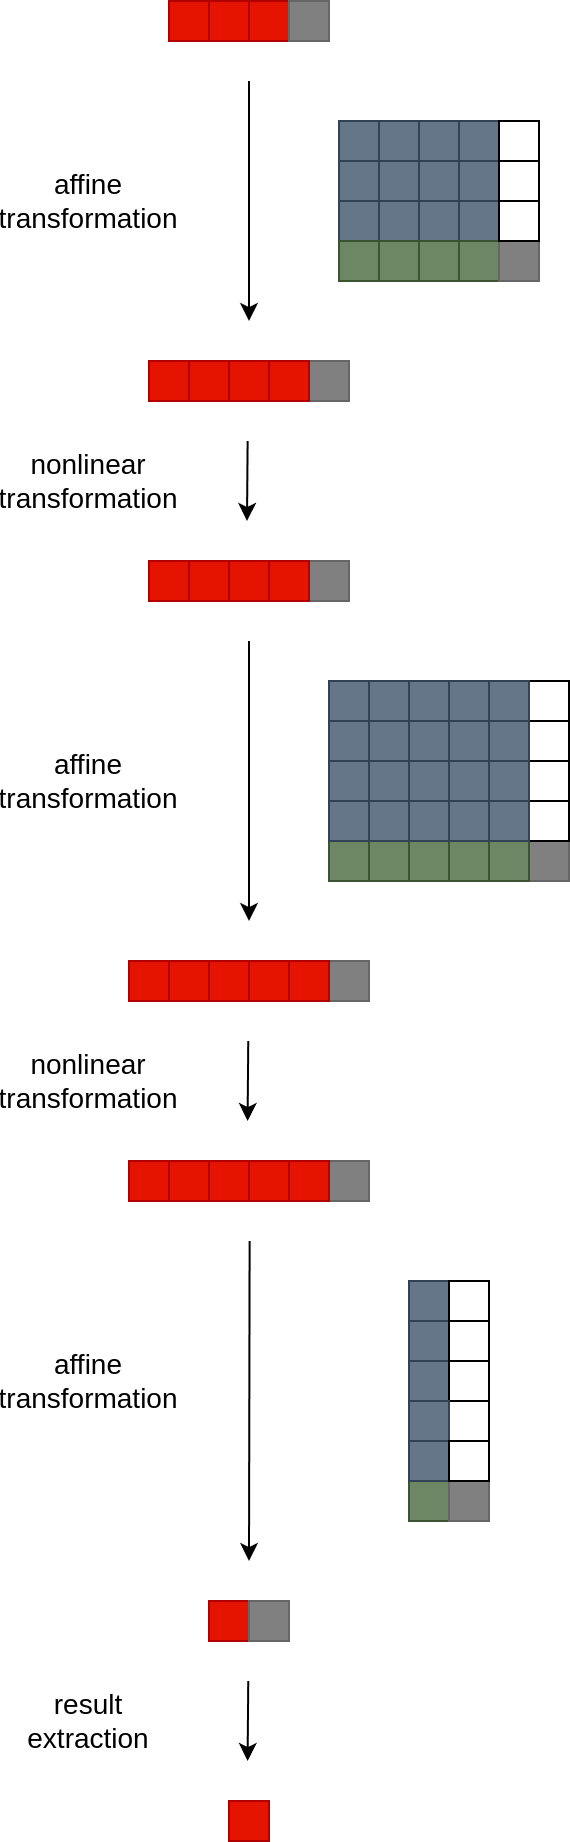
\includegraphics[scale=0.3]{../images/nn.png}
	\caption{Neural network illustration}
    \label{fig:nn}
\end{figure}

\subsection{Tree-based genetic programming}

Tree-based genetic programming (TBGP) \citep{tbgp} encodes a symbolic expression in a tree format. An illustration of TBGP for an expression for the function $x^2 + xy +2x - y$ is shown in figure \ref{fig:tbgp}. This function will be used as an example in all the remaining algorithms as well.

The creation operator creates a random tree. At each node, it has a chance of generating a parameter, a constant, or a function onde. The combination operator selects a random subtree in the first parent, and replaces it with a random subtree from the second parent. The perturbation operator selects a random subtree in the parent, and replaces it with a randomly generated subtree, which is generated using the creation operator. The regression algorithm evaluates the tree as an expression.

Hyperparameters for TBGP are the maximum height of a tree, the chance of generating a parameter leaf, and the chance of generating a constant leaf.

\begin{figure}[!htbp]
	\centering
	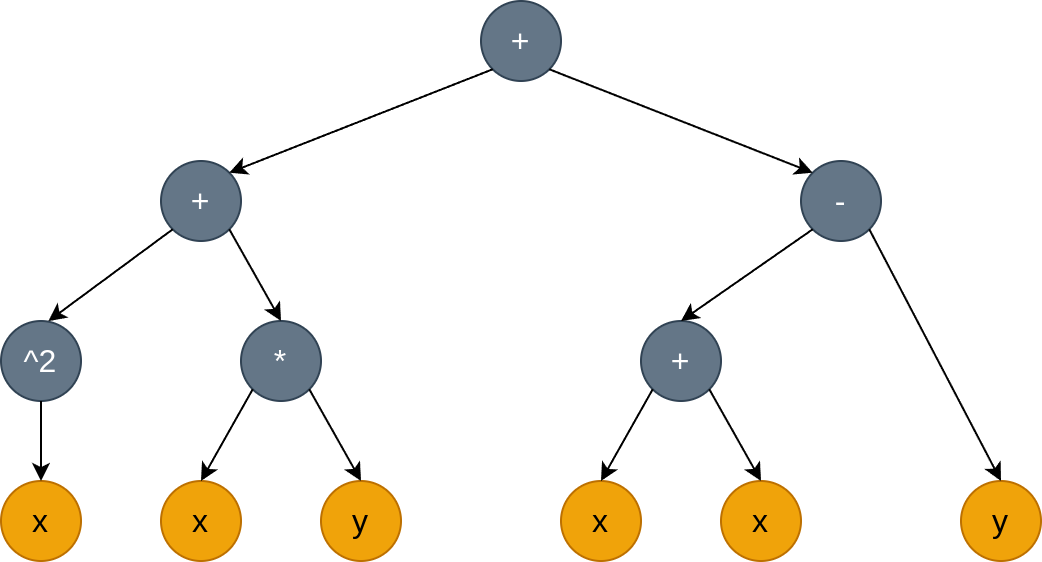
\includegraphics[scale=0.3]{../images/tbgp.png}
	\caption{Tree-based genetic programming illustration}
    \label{fig:tbgp}
\end{figure}

\subsection{Cartesian genetic programming}

Cartesian genetic programming (CGP) \citep{cgp} encodes a symbolic expression in a two-dimensional grid of function nodes. Since functions may not have the same arity, each node has the number of arguments which is equal to the maximum arity across all functions. The output of the grid can be chosen as any of the grid elements, or any of the inputs. An illustration of CGP is shown in figure \ref{fig:cgp}.

The creation operator creates a random grid. The combination operator generates a random breakpoint in the grid, and it copies the part from the start to the breakpoint from the first parent, and the part from the breakpoint to the end from the second parent. This scheme is often called \textit{one-point crossover}. The mutation operator selects $k$ random nodes, and either changes their function, or their arguments. The regression algorithm evaluates all grid elements, column by column, and the output is taken from the output node. This algorithm can be optimized using top-down dynamic programming.

Hyperparameters for CGP are the number of rows, number of columns, and the perturbation rate, which encodes the percentage of grid nodes which will be changed by the perturbation operator.

\begin{figure}[!htbp]
	\centering
	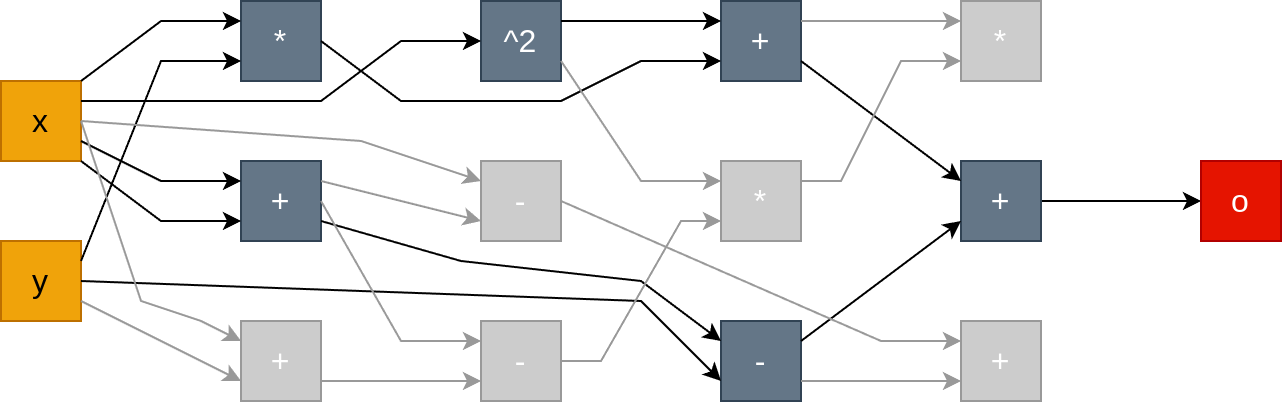
\includegraphics[scale=0.3]{../images/cgp.png}
	\caption{Cartesian genetic programming illustration}
    \label{fig:cgp}
\end{figure}

\subsection{Graph-based genetic programming}

Graph-based genetic programming (GBGP) encodes a symbolic expression in a directed acylcic graph. An illustration of GBGP is shown in figure \ref{fig:gbgp}. Representation and perturbation operator for GBGP were derived from \citep{gbgp}, while the combination operator for GBGP was derived from \citep{gbgp_operators}.

The creation operator creates a random graph. The combination operator selects a random subgraph in the first parent, and replaces it with a random subgraph from the second parent. The perturbation operator deletes a random amount of nodes, inserts a random amount of nodes, and changes either the function or the arguments for a random amount of nodes. The regression algorithm evaluates the expression encoded in the graph, and is very similar to the regression algorithm for CGP.

Hyperparameters for GBGP are the maximum number of nodes, perturbation rate, maximum number of nodes to delete during perturbation, maximum number of nodes to insert during perturbation, maximum number of nodes to crossover during combination, and the chance of proceeding to a predecessor of a node, which is used when selecting subgraphs during combination.

\begin{figure}[!htbp]
	\centering
	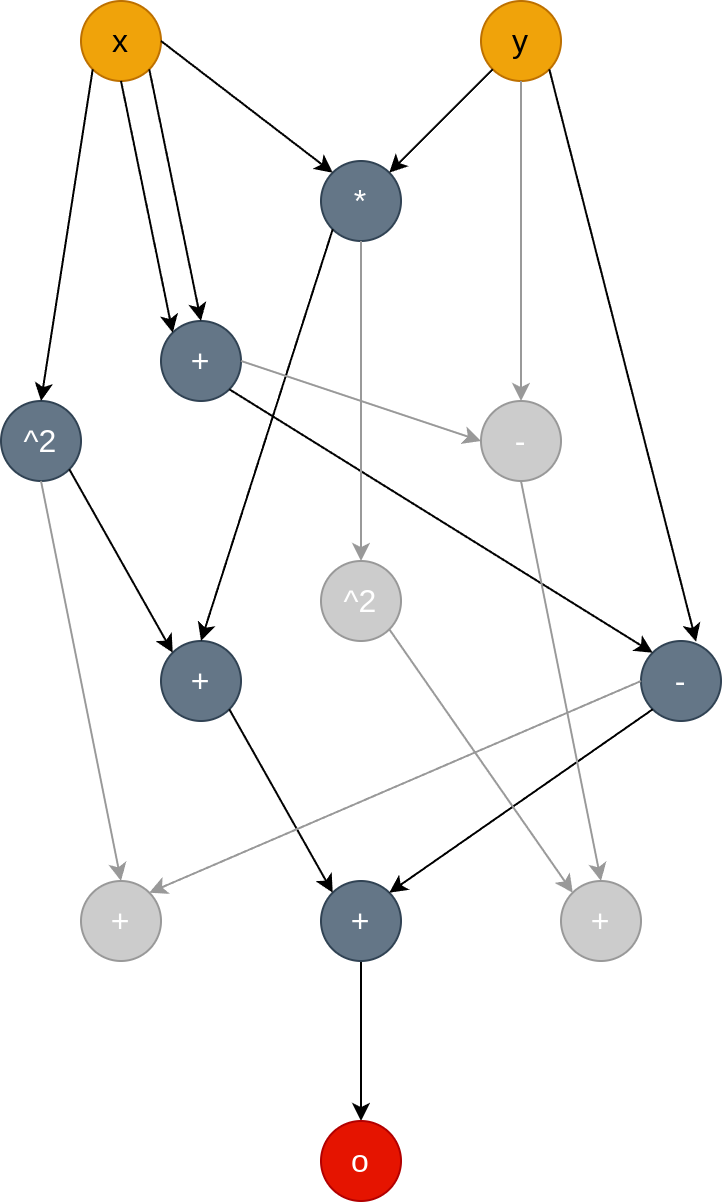
\includegraphics[scale=0.3]{../images/gbgp.png}
	\caption{Graph-based genetic programming illustration}
    \label{fig:gbgp}
\end{figure}

\subsection{Stack-based genetic programming}

Stack-based genetic programming (SBGP) \citep{sbgp} encodes a symbolic expression in the Reverse Polish Notation (RPN). A few rules are needed to ensure that the program execution is always valid. If the top element of the stack is a function, and it does not have enough arguments on the stack, then it is removed from the stack without any further manipulations. If the stack is empty when the evaluation finishes, then the value $0$ is returned instead of an error. An illustration of SBGP is shown in figure \ref{fig:sbgp}. The set of instructions is shown on the left, and the state of the stack after each operation is shown on the right of the figure. The number of instructions is fixed, and empty instructions are encoded as \textit{NOP (no operation)}, to functionally allow programs to have different lengths.

The creation operator creates a random expression in RPN. The combination operator is the one-point crossover. The perturbation operator randomly selects some functions and replaces them with different functions. The regression algorithm evaluates the expression using a stack.

Hyperparameters for SBGP are the number of instructions, chance of \textit{NOP} during creation, chance of \textit{NOP} during perturbation, the chance of generating a \textit{PUSH <constant>} instruction, the chance of generating a \textit{PUSH <parameter>} instruction, and the perturbation rate.

\begin{figure}[!htbp]
	\centering
	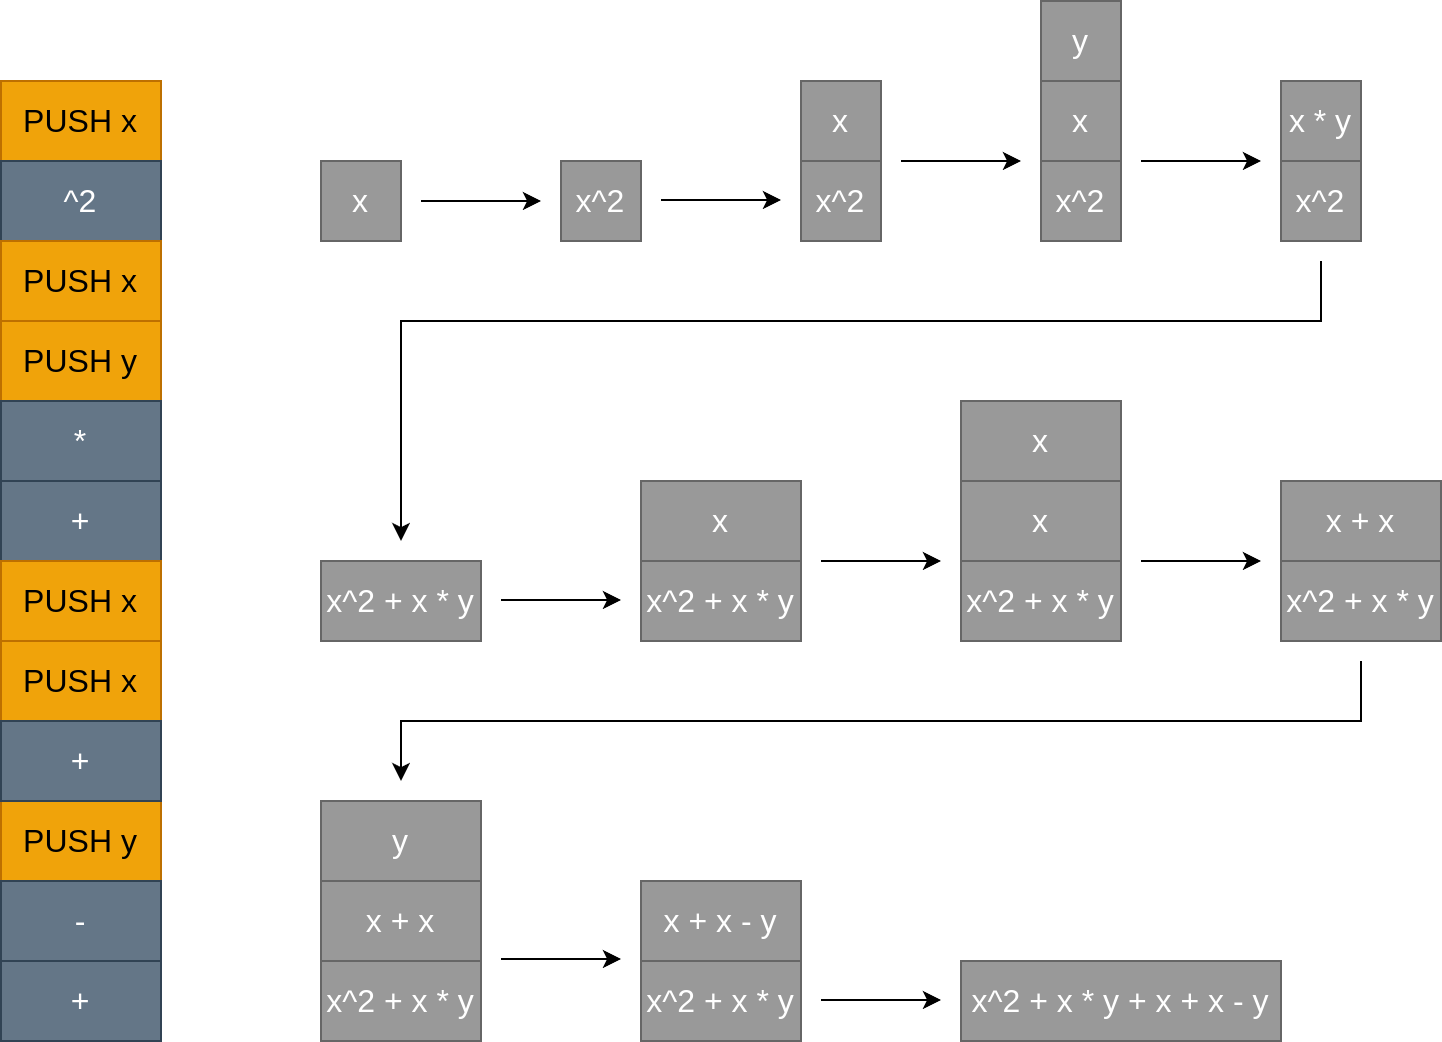
\includegraphics[scale=0.28]{../images/sbgp.png}
	\caption{Stack-based genetic programming illustration}
    \label{fig:sbgp}
\end{figure}

\subsection{Linear genetic programming}

Linear genetic programming (LGP) \citep{lgp} encodes a symbolic expression in an imperative program, containing instructions which resemble a RISC architecture. Similar to SBGP, programs have a fixed number of instructions, but some of these instructions can be empty \textit{NOP} instructions. An illustration of LGP is shown in figure \ref{fig:lgp}. The set of instructions is shown on the left, and the state of registers after each operation is shown on the right.

The program has a fixed number of registers to work with. Registers can be initialized in several ways:
\begin{itemize}
	\item empty - all registers are initialized to zero
	\item singular - first $k$ registers are initialized to $k$ parameters, and the remaining registers are initialized to zero
	\item circular - all registers are initialized in a round-robin way, using parameters
\end{itemize}

The creation operator creates a random program. The combination operator is the one-point crossover. The perturbation operator randomly selects some instructions and changes either their type or their arguments. The regression algorithm executes the program and returns the value in the first register.

Hyperparameters for LGP are the number of instructions, number of registers, register initialization strategy, chance of \textit{NOP} during creation, chance of \textit{NOP} during perturbation and the perturbation rate.

\begin{figure}[!htbp]
	\centering
	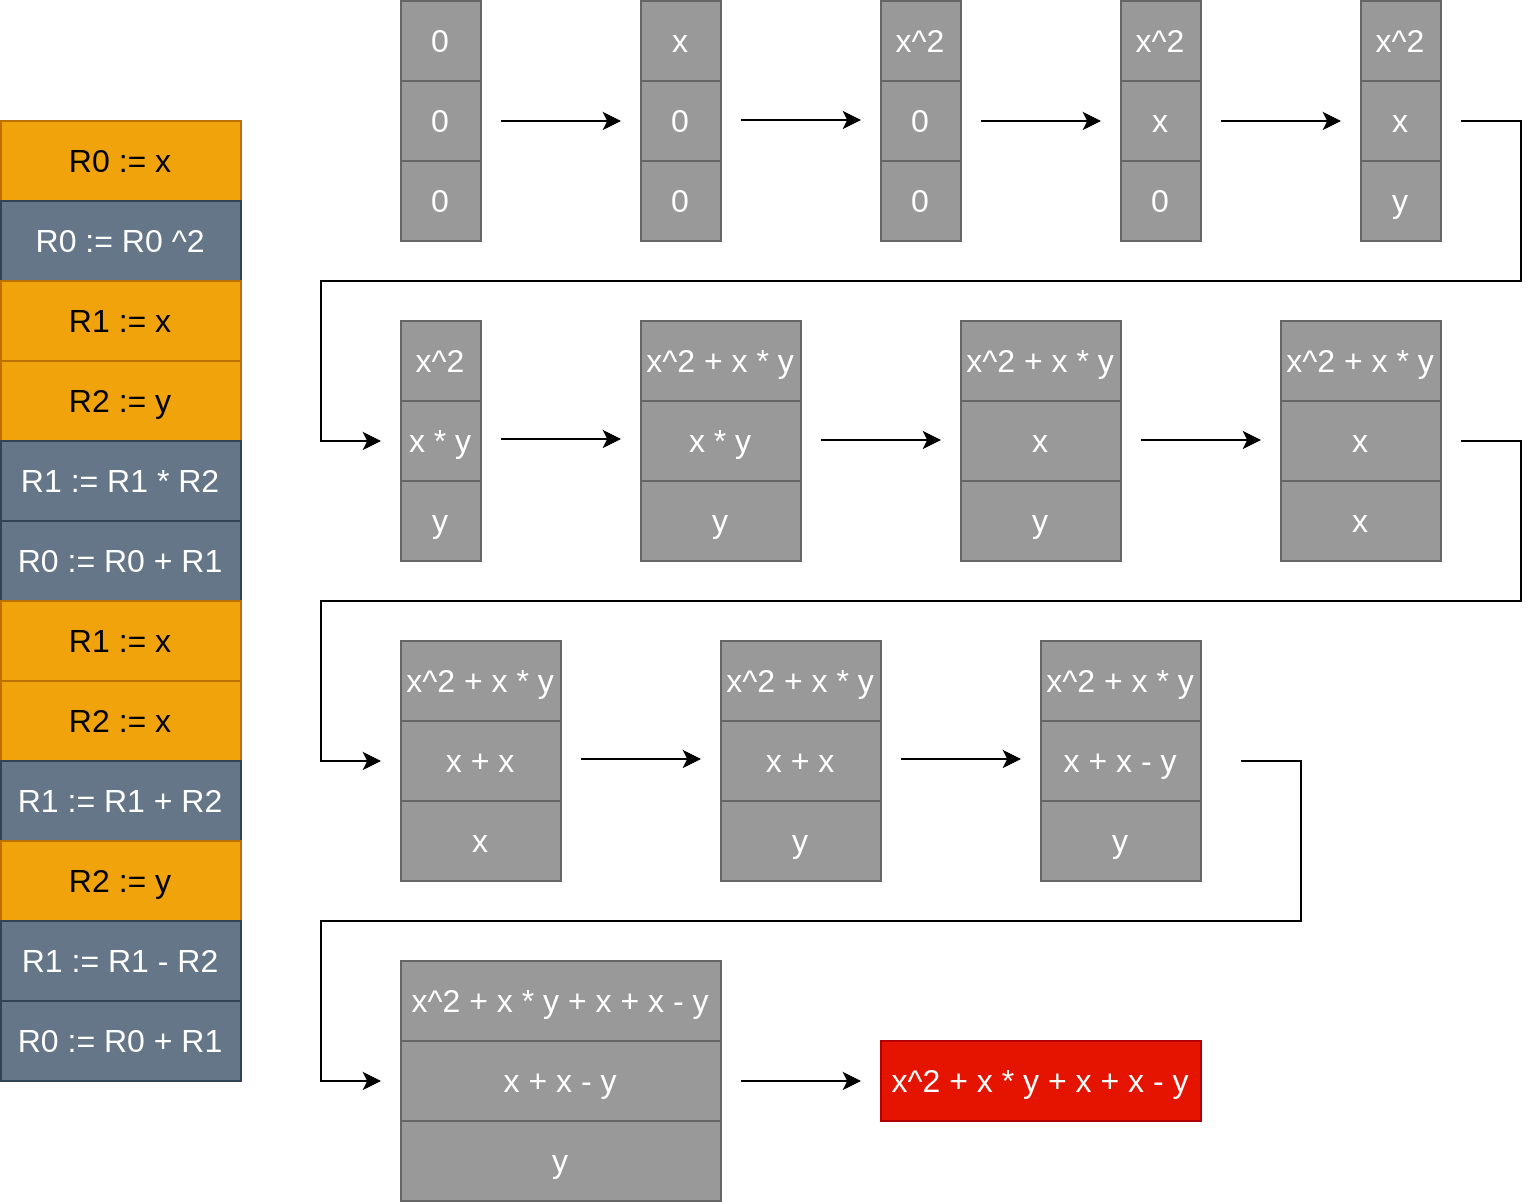
\includegraphics[scale=0.25]{../images/lgp.png}
	\caption{Linear genetic programming illustration}
    \label{fig:lgp}
\end{figure}

\subsection{Multi expression programming}

Multi expression programming (MEP) \citep{mep} encodes several symbol expressions, where expressions are built using the previous expressions, and any one of them can be used as the solution for the problem. To adapt this algorithm to be usable for online scheduling, we will always use the last expression as the result for the regression problem. An illustration of MEP is shown in figure \ref{fig:mep}.

The creation operator creates a random program. The combination operator is the one-point crossover. The perturbation operator randmoly selects some expressions and changes their arguments or function. The regression algorithm evaluates all expressions and uses the last one as the result.

Hyperparameters for MEP are the number of instructions and the perturbation rate.

\begin{figure}[!htbp]
	\centering
	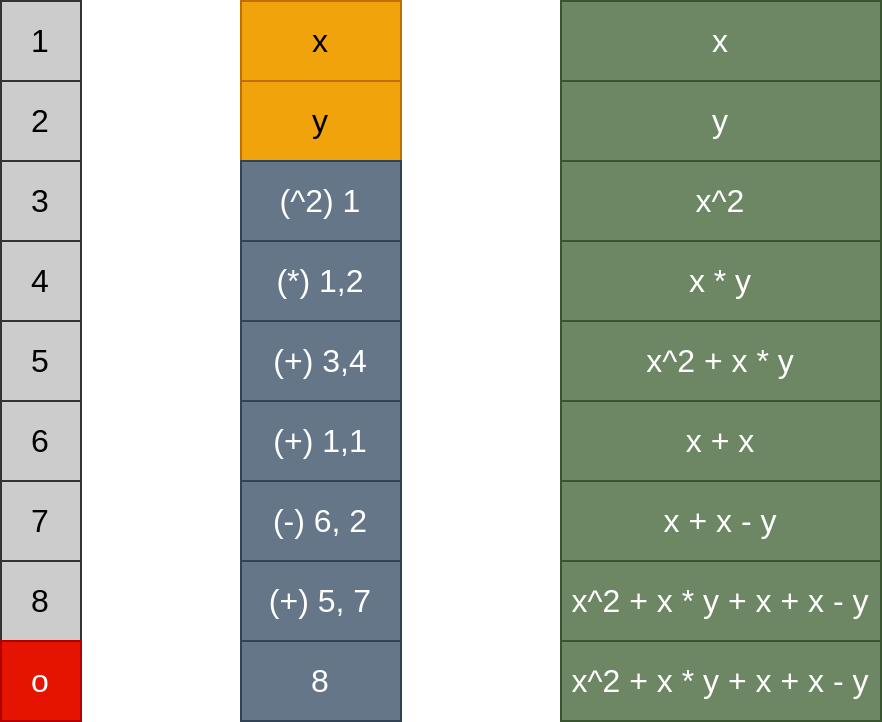
\includegraphics[scale=0.3]{../images/mep.png}
	\caption{Multi expression programming illustration}
    \label{fig:mep}
\end{figure}

\subsection{Gene expression programming}

Gene expression programming (GEP) \citep{gep} has distinct representations for its genotype and phenotype. The genotype is a linear string of elements, which can be either function symbols, parameters or constants. The phenotype is constructed by using the genotype to build the expression tree, level by level. The genotype consists of two parts, head and tail. The head can contain function symbols, while the tail cannot. The length of the head is a hyperparameter of the algorithm, and the length of the tail is calculated from the head's length. This ensures that the resulting expression is always valid and complete. And illustration of GEP is shown in figure \ref{fig:gep}.

The creation operator creates a random genotype string. The combination operator is the one-point crossover. The perturbation operator randomly selects some genotype elements and changes them, and also randomly performs transposition, which selects a segment of the genotype, and moves it to a different position within the genotype. The regression algorithm build the phenotype tree from the genotype, and then evaluates the expression encoded in the tree.

Hyperparameters for GEP are the head size, the chance of generating a parameter in the tail (as opposed to a constant), perturbation rate, chance of transposition happening in perturbation, and the maximum length of the segment in the transposition.

\begin{figure}[!htbp]
	\centering
	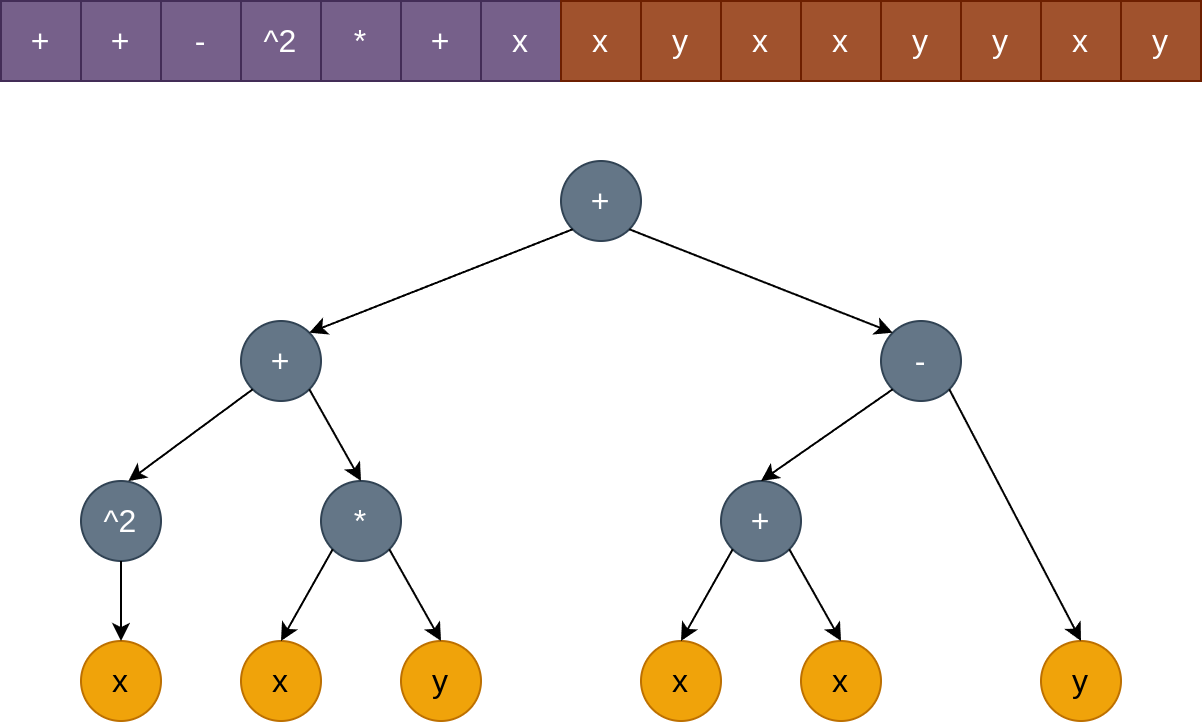
\includegraphics[scale=0.3]{../images/gep.png}
	\caption{Gene expression programming illustration}
    \label{fig:gep}
\end{figure}

\subsection{Grammatical evolution}

Grammatical evolution (GE) \citep{ge} is another algorithm with distinct representations for genotype and phenotype. The genotype is a linear string of integers called codons, and the phenotype is an expression tree. The phenotype tree is constructed from the genotype string using a context-free grammar and the modulo operator. Each time that a production is used, one codon is consumed. When all codons are consumed, the mapping starts from the beginning, and this process is called wrapping. The number of wrappings should be limited. In some cases, the mapping from genotype to phenotype may not be successful, for example due to loops. In this case, the authors of the algorithm propose assigning the lowest possible fitness value to the individual. However, this is not applicable in the case of scheduling, where it takes several evaluations of an online scheduling algorithm before the whole system can be evaluated. Instead, if the phenotype construction fails, the algorithm will always return a constant value $0$. An illustration of GE is shown in figure \ref{fig:ge}.

The creation operator creates a random genotype string. The combination operator is the one-point crossover. The perturbation operator randomly selects some codons and changes their values. The regression algorithm builds the phenotype tree from the genotype, and then evaluates it as an expression.

Hyperparameters for GE are the codon count, the maximum number of wrappings, and the perturbation rate.

\begin{figure}[!htbp]
	\centering
	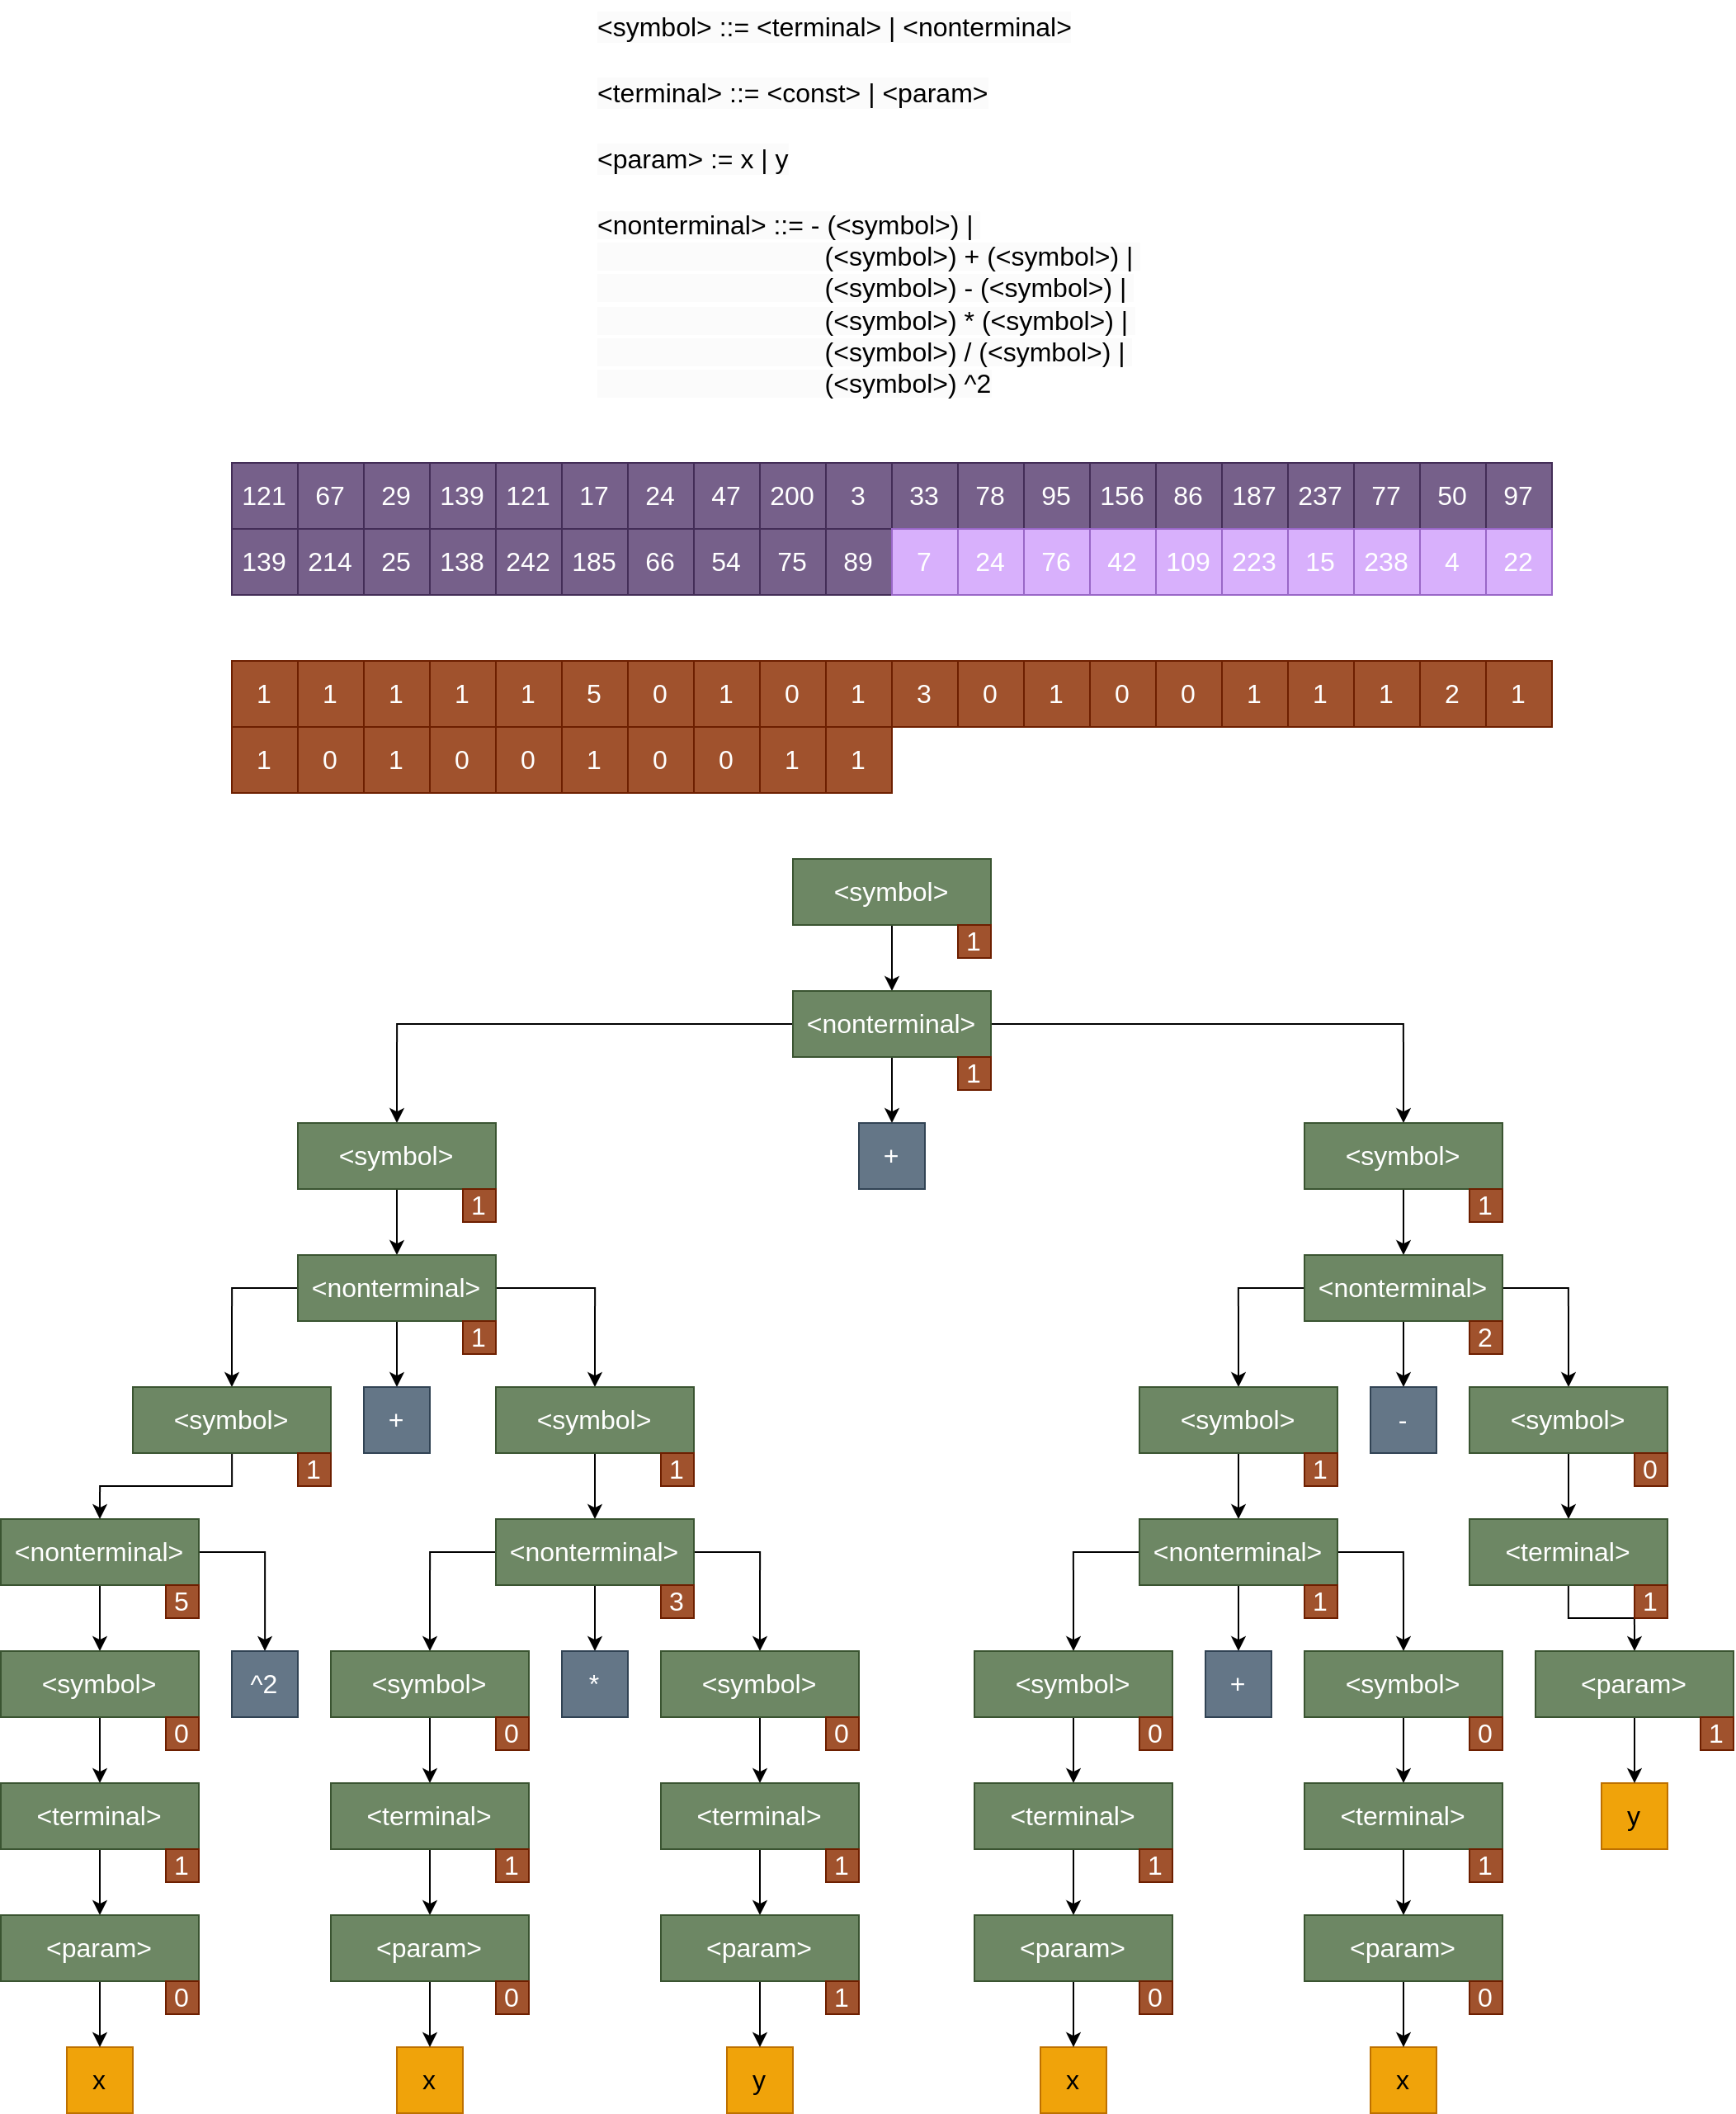
\includegraphics[scale=0.19]{../images/ge.png}
	\caption{Grammatical evolution illustration}
    \label{fig:ge}
\end{figure}

\subsection{Structured grammatical evolution}

Structured grammatical evolution (SGE) \citep{sge} is an algorithm inspired by the GE. It solves the problem of the mapping from genotype to phenotype possibly failing, by limiting the depth of the tree. For each nonterminal symbol in the grammar, it keeps a linear string of codons, whose length is equal to the maximum number of times that a symbol could appear in any tree, with the given maximum depth. An illustration of SGE is shown in figure \ref{fig:sge}. The maximum depth here is three, and the source of the recursion in the grammar is the $symbol$ node being mapped to a combination of $nonterminal$ nodes and an operator. In this case, after this transformation is applied three times in any path from the root of the tree to its leaves, the $symbol$ node will always be mapped to the $terminal$ node, thus ending the recursion.

The creation operator creates random genotype strings, one for each nonterminal symbol. The combination operator follows this procedure for each nonterminal symbol - choose a random parent, and copy its genotype for the nonterminal symbol to the child. The perturbation operator randomly selects some codons and changes their values. The regression algorithm build the phenotype tree from the genotype, and then evaluates it as an expression.

Hyperparameters for SGE are the maximum depth and the perturbation rate.

\begin{figure}[!htbp]
	\centering
	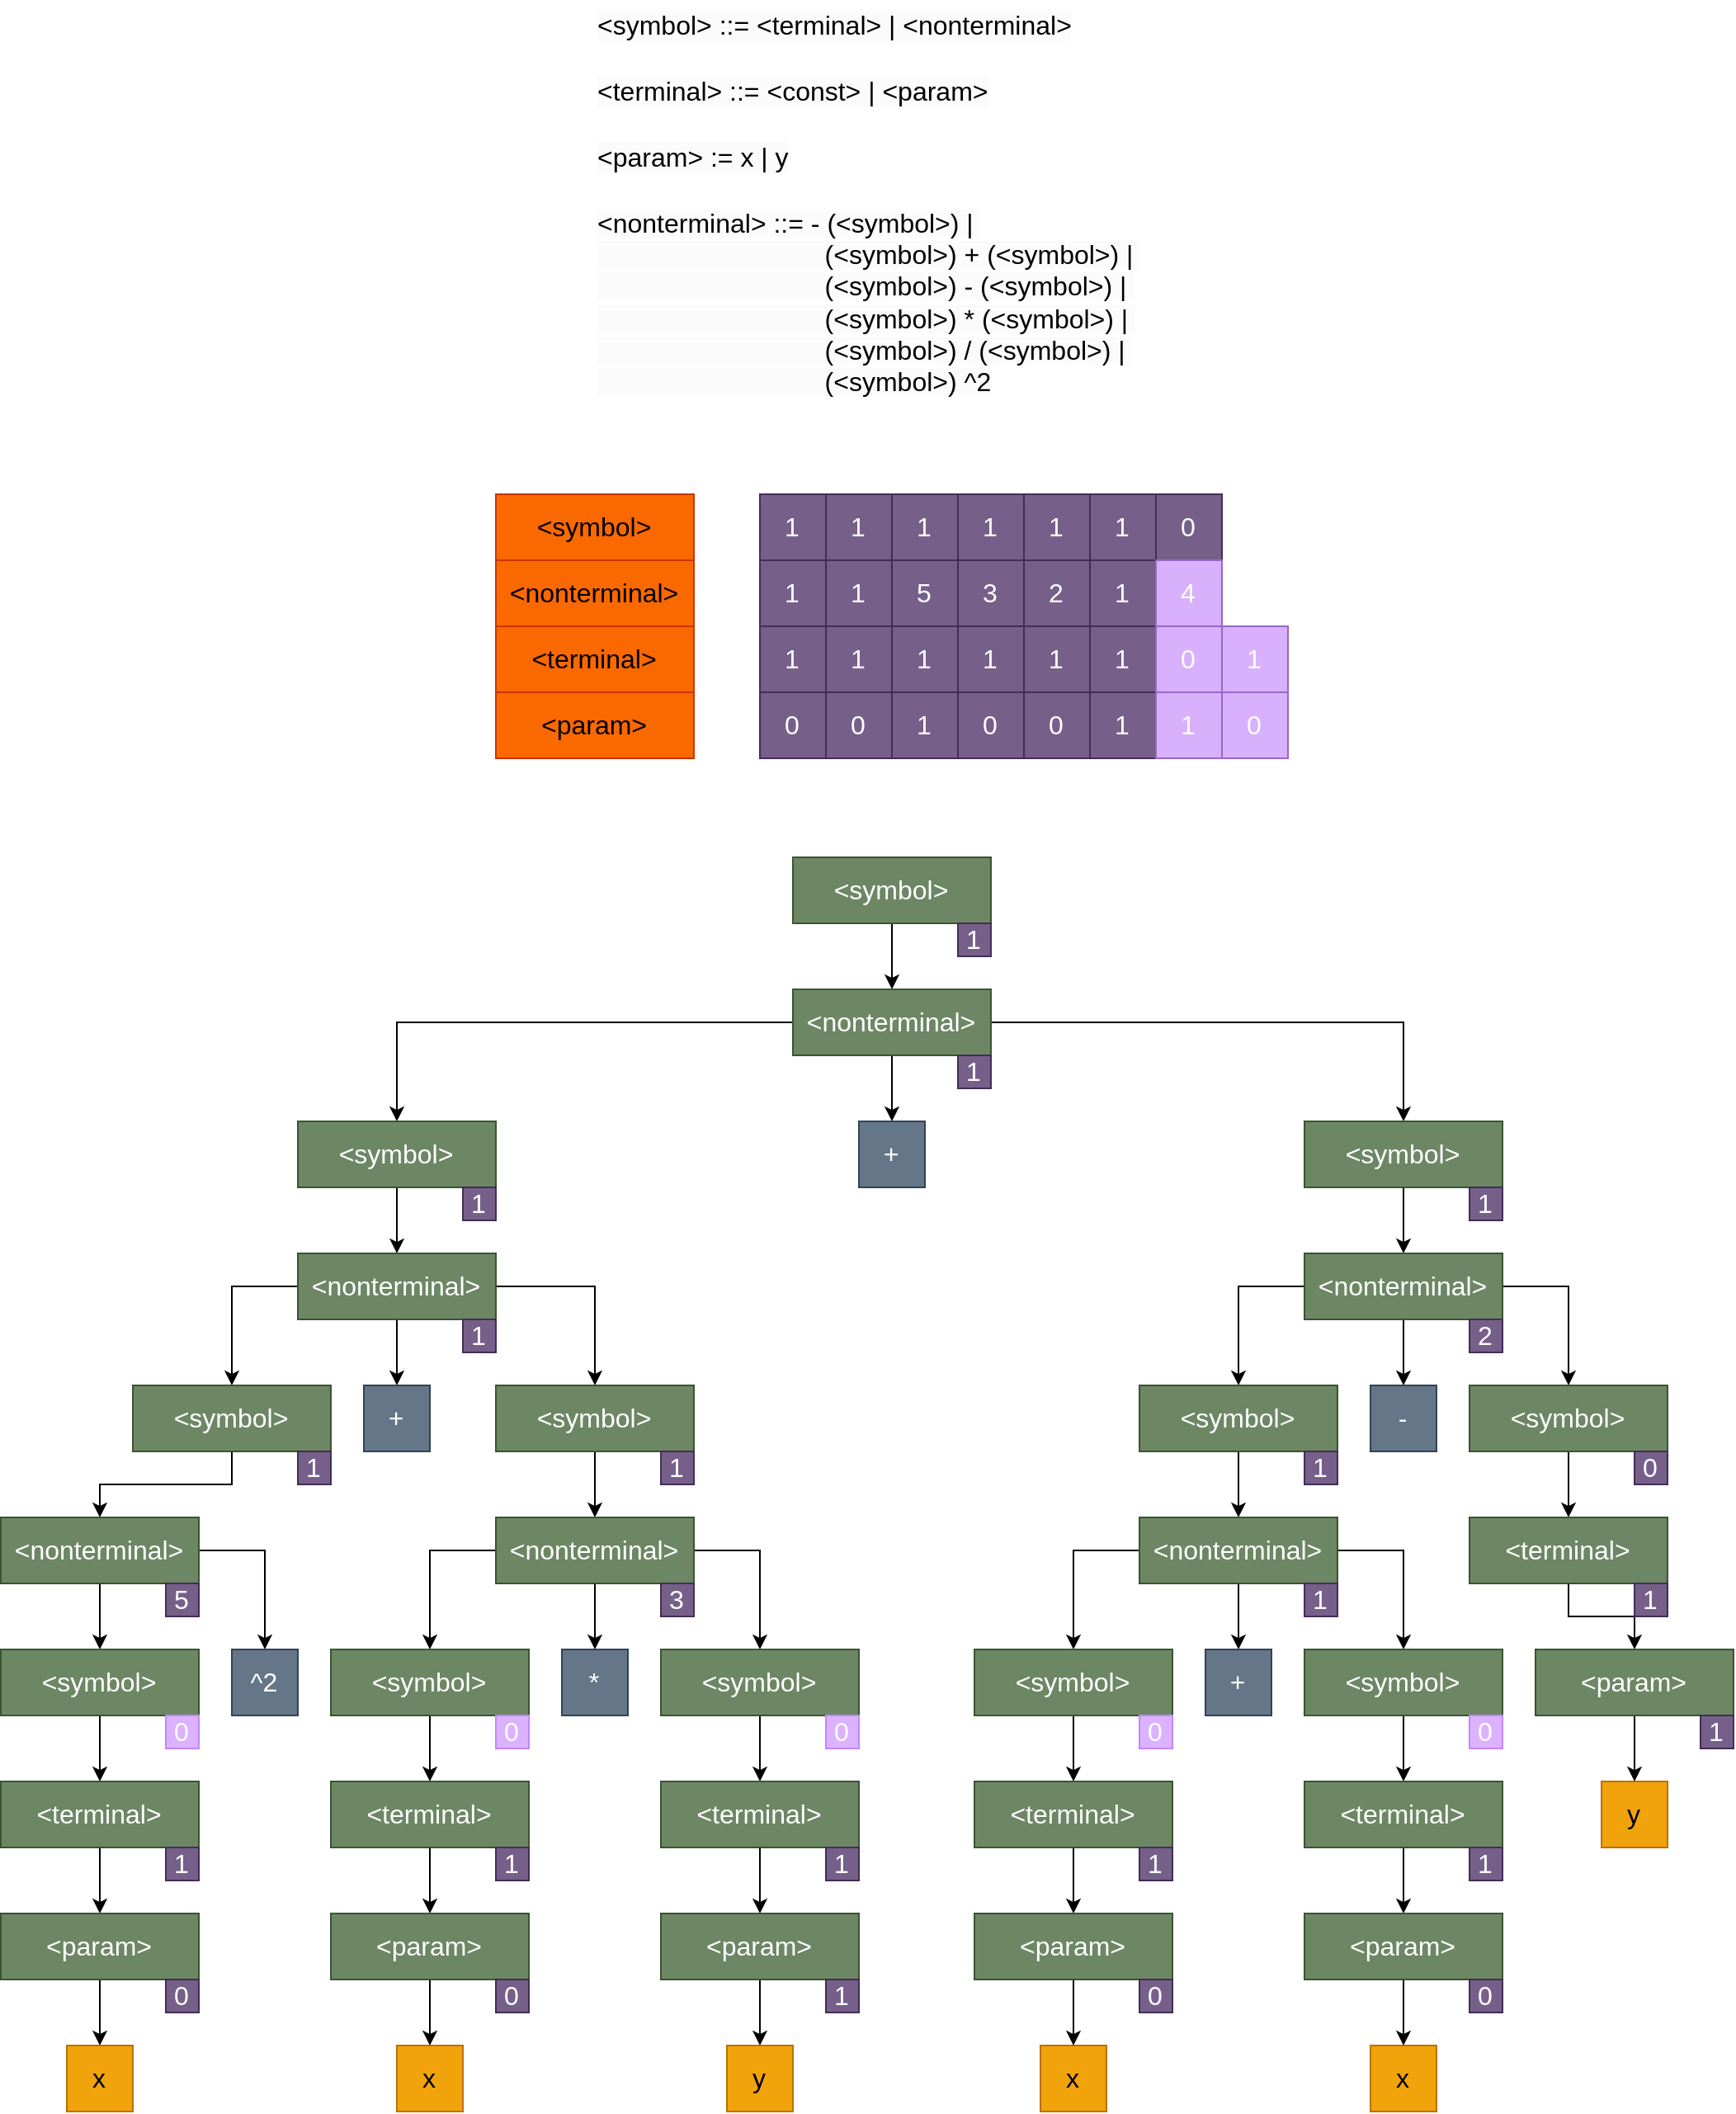
\includegraphics[scale=0.19]{../images/sge.png}
	\caption{Structured grammatical evolution illustration}
    \label{fig:sge}
\end{figure}